% Benvenuti nel template per le relazioni di Sperimentazioni di Fisica 1 del corso triennale in Astronomia dell'Università di Padova.
% Per compilarlo, cliccate su Menu, selezionate come compilatore "pdfLaTeX", TeX Live Version 2020 (o uno degli altri, whatever works), e come documento principale "Relazione.tex"

%%% Preambolo del documento %%%
% Non toccate questa roba, a meno che non siate abbastanza sgamati da sapere quello che state facendo, tipo vi piacciono di più certi pacchetti rispetto ad altri, o magari ve ne manca qualcuno.
\documentclass[a4paper, titlepage]{article}
\usepackage[T1]{fontenc}
\usepackage[utf8]{inputenc}
\usepackage[english]{babel}
\usepackage{amsmath}
\usepackage{listings}
\usepackage{textcomp}
\usepackage{multirow}
\usepackage{multicol}
\usepackage{booktabs}
\usepackage{graphicx}
\usepackage{floatflt}
\usepackage{epsfig}
\usepackage{pstricks}
\usepackage{subfigure}
\usepackage[labelfont=bf, font=scriptsize]{caption}
\usepackage[english]{varioref}
\usepackage[suftesi]{frontespizio}
\usepackage{color}
\usepackage{tikz}
\usepackage{caption}
\usepackage{pgfplots}
\usepackage{comment}
\usepackage{lipsum}
\pgfplotsset{compat=1.16}
\usepackage{listings} %red, green, blue, yellow, cyan, magenta, black, white
\definecolor{mygreen}{RGB}{28,172,0} % color values Red, Green, Blue
\definecolor{mylilas}{RGB}{170,55,241}

\lstset{language=Matlab,%
    %basicstyle=\color{red},
    breaklines=true,%
    morekeywords={matlab2tikz},
    keywordstyle=\color{blue},%
    morekeywords=[2]{1}, keywordstyle=[2]{\color{black}},
    identifierstyle=\color{black},%
    stringstyle=\color{mylilas},
    commentstyle=\color{mygreen},%
    showstringspaces=false,%without this there will be a symbol in the places where there is a space
    numbers=left,%
    numberstyle={\tiny \color{black}},% size of the numbers
    numbersep=9pt, % this defines how far the numbers are from the text
    emph=[1]{for,end,break},emphstyle=[1]\color{red}, %some words to emphasise
    %emph=[2]{word1,word2}, emphstyle=[2]{style},    
}

%%% Il documento vero e proprio %%%
\begin{document}

%%% Frontespizio %%%
% Questa serie di comandi genera il frontespizio della relazione.
% Cambiate: l'Anno Accademico, Data e Titolo della relazione, il nome degli appartenenti al gruppo con annessa matricola e mail istituzionale. Se siete due o quattro in gruppo, basta togliere/inserire una riga Candidato.
% NON toccate i comandi con accanto con CTT (Can't Touch This).
% !!! NOTA PER LA CORRETTA VISUALIZZAZIONE DEL FRONTESPIZIO. !!!
% Quando si compila un file su Overleaf, per velocizzare le successive compilazioni questi genera una cache, e da questa prende gli elementi che, a senso suo, non sono cambiati nel testo. Quindi per quanto vi possiate ostinare a compilare, vedrete sempre il primo frontespizio che ha compilato (quello con NomeCognome etc etc) e non le ultime modifica.
% Come evitare ciò, e visualizzare il frontespizio con i vostri nomi, cognomi e numeri matricola? Così: cliccate sull'icona accanto a Recompile, quella con il simbolo del documento, e successivamente sul simbolo del cestino (Clear cached files). Liberate la cache, modificate il frontespizio, e ricompilate. Così dovreste riuscire a vedere nel file compilato le vostre modifiche al frontespizio. Ricordatevi di svuotare la cache del file Overleaf ogni volta che volete modificare qualcosa nel frontespizio.
\begin{frontespizio}
\Universita{Padova} % CTT
\Logo{Figure/logo_unipd} % CTT
\Divisione{Neurorobotics and Neurorehabilitation A.A. 2020 2021} % CTT
\Corso[Masters'degree]{Computer engineering} % CTT, a meno che non cambi la denominazione del corso
\Annoaccademico{2020-2021+1}
\Titoletto{Project 5} % CTT
\Titolo{Longitudinal analyses on MI BMI data}
\Sottotitolo{09 September 2021}
\NCandidati{Team} % CTT
\Candidato[2005833]{Francesco Agostini, \textsf {francesco.agostini.5@studenti.unipd.it}}
\NRelatore{Teacher}{} % CTT
\Relatore{Prof. Luca Tonin} % CTT, a meno che non sia cambiato il Prof.
\Relatore{Prof. Emanuela Formaggio} % CTT, a meno che non sia cambiato il Prof.
\Relatore{Prof. Maria Rubega} % CTT, a meno che non sia cambiato il Prof.
\end{frontespizio}
\IfFileExists{\jobname-frn.pdf}{}{%
\immediate\write18{pdflatex \jobname-frn}} % ASSOLUTAMENTE CTT, è il comando che materialmente vi genera il frontespizio.

%%% Indice %%%
\tableofcontents

\newpage
%%% Sezioni %%%
% Qui inizia la relazione vera e propria.
% Le Sezioni sono singoli file .tex dentro la cartella Sezioni. Potete a libera scelta scrivere tutto su un singolo file e chiamare all'interno di questi con il comando \section{} le varie sezioni, oppure dividere le singole sezioni in più file Sezione_i.tex, e poi inserirle tutte con \input{Sezioni/Sezione_i.tex} per i = 1 ... N
% Titolo della sezione e label. Vi consiglio, per questioni di ordine mentale e rapidità successiva di reference, di etichettare le label in modo sensato, con riferimento chiaro a cosa si sta etichettando. Quindi sec:nomesezione per una sezione, im:nomeimmagine per una immagine, e via dicendo.
\section{Introduction}\label{sec:introduction} 
The Project 5 is a real application of the techniques of EEG signal processing studied in class on a real case. 
\subsection{Description of the case}\label{subsec:desc}
The case is the 2019 Cybathlon race, where a pilot have to interact with a game using a BMI, the pilot use 2 motor imagery to control the game interface. The motor imagery is both hands and both feet. In a period of 3 month the pilot in 11 sessions performed two kinds of runs. Offline where the pilot not have real feedback, used only for calibration, and Online session where pilot receive visual stimulus as a feedback of his commands. The pilot on the online runs can see on the screen two colored bars related to the imagery tasks. The colored bars is filled according with the output of the classifier on actual signals.
\subsection{Data Description}\label{subsec:datadesc}
The 11 sessions are composed with some gdf file, containing all information regarding the run type and ordered by timestamp:
\begin{itemize}
    \item \textbf{$20190502_F1$} Executed in 02nd of May 2019 and composed by 3 offline runs and 3 online runs.
    \item \textbf{$20190506_F1$} Executed in 05th of May 2019 and composed by 1 long offline runs and 5 online runs.
    \item \textbf{$20190513_F1$} Executed in 13th of May 2019 and composed by 1 long offline runs and 3 online runs.
    \item \textbf{$20190521_F1$} Executed in 21th of May 2019 and it started with an online run, followed by 3 offline runs and closed with a last online run.
    \item \textbf{$20190610_F1$} Executed in 06th June 2019 and composed only by an online run. 
    \item \textbf{$20190624_F1$} Executed in 24th June 2019 and composed only by an online run. 
    \item \textbf{$20190627_F1$} Executed in 27th June 2019 and composed only by an online run. 
    \item \textbf{$20190701_F1$} Executed in 1st July 2019 and composed by 7 online runs. 
    \item \textbf{$20190709_F1$} Executed in 9th July 2019 and started with 2 online runs followed by 4 offline runs anc closed with a last online run. 
    \item \textbf{$20190711_F1$} Executed in 11th July 2019 and composed by 2 online runs. 
    \item \textbf{$20190715_F1$} Executed in 15th July 2019 and composed by 2 online runs. 
\end{itemize}
\newpage
\subsection{Pipeline description}\label{subsec:pipeline}
For this project the first important thing to do is configure the project with fundamental parameter used for all tasks, after that we can proceed loading data session keeping divided for each session online data from offline data. The main idea is to analyze offline sessions before computing fisher score and extracting channel and frequencies that could be used as discriminant for the classifier, create a classifier for each session, test classifiers with online runs measuring the performance. On Figure 1 we can see the 4 main component that compose the pipeline. I used factory/builder pattern to approach the problem, During the first phase we have to process data in order to identify a good discriminant for feature selection, during this phase we'll use only the first part of the pipeline for analyze offline sessions. Only in the second phase after feature selection will use the complete pipeline. 
\begin{figure}[h]
    \centering
    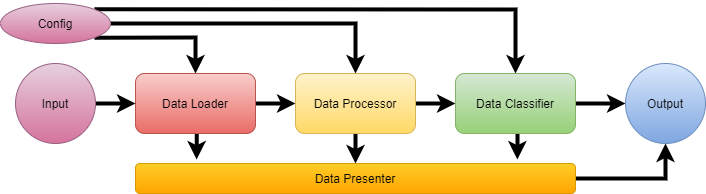
\includegraphics[width=0.8\textwidth]{Figure/NR_Pipeline.png}
    \caption{Pipeline description.}
    \label{fig:Pipeline}
\end{figure}\\
\begin{itemize}
    \item Data Loader: Responsible of data loading and early processing. This component is a standalone class with collection container for the data in the gdf files. Another important responsibility of this class is the early data processing with spatial filtering and spectrogram computing.
    \item Data Processor: The class responsible for the data processing and manipulation during analysis procedure. This class do all step necessary to extract the information necessary for the feature selection and classifier training. 
    \item Data Classifier: This is the last component of the pipeline, another class with all method necessary for the dataset (trainset and testset) and classifier train test operation.
    \item Data Presenter: The only class of the pipeline parallel to all component with only static methods. Each component of the pipeline have a reference to this class, in order to call necessary method to plot output and chart. This component of the pipeline not have class member except the output configuration.
\end{itemize}
The pipeline was created for allow to each module easy access to output of previous module. Data processor has a reference of data loader class for get data, and data classifier have a reference to data processor. With this method each component can easily access to the past history of the data.

	
\section{Methods}\label{sec:Methods} 
All method used in this pipeline come from the classroom exercise and home works. But are organized and structured in order to work with different datasets just changing configuration on the main script and inserting session data in the right place.
\subsection{Cofiguration}\label{subsec:configuration}
For this project following the data specification we choose the following configuration parameter. The first part of the configuration is used to set the necessary parameter to spectrogram computation. The second part of the config is dedicated to the classifier setup after feature selection procedure in phase 1. The last config part is dedicated to the Data Presenter class, and allow to choose which plot show during pipeline.
Datapath var is the root source data folder that will used by the project, and var f is the frequency vector (from:step:to)

\lstinputlisting{Figure/Code/config.m}


\subsection{Data Loading}\label{subsec:loading}
Data loading procedure starts looking with listSession() function for all subfolder in datapath, exluded . and .. for obvious reason. Each folder contained in datapath will be considered a session for the system and will be sorted by name. In our case with the timestamp at the beginning of each session folder the system will be sort in chronological order. After session listing the DataLoader class procede iterating each session (folder) with loadSessions() function and start to load the each session with loadSession() function. 

\subsection{Data Chaining}\label{subsec:status}
The loadSession() function start enumerating all gdf files and procede loading gdfs file using sload function. For each runs the function use the preprocessing function in order to do spatial filter operation and spectrogram computing. After this preprocessing operation the function chain all event vectors TYP (type) DUR(Duration in sample) POS(Position in sample). Keeping splitted offline runs from online runs. These information are stored as class member with name sessionsDataOffline(sessionIndex) that contain all chained data of offline runs, and sessionsDataOnline(sessionIndex) that contain all online runs information.
\subsection{Spatial Filtering}\label{subsec:spatial}
For the spatial filtering the laplacian filter is used with function contained in laplacian16.mat file. This operation is necessary for a better comprension of data across the EEG channels during the spectrogram computation. In fact differently from Common average reference tecnique that introduce 'noise' from near channels, laplacian filtering approssimate the 2nd order derivative subtracting the mean acrivity of the neighbor channels. The result is an highlited spatial location of SMR.   
\subsection{Spectrogram and PSD}\label{subsec:psd}
Using the spectrogram compute function provided in clas,s the spectrogram of each run is computed and stored in vector named P, as TYP DUR POS events information, the spectrogram vector are chained and inserted in the appropriate online/offline session vector, ready to be used from the next step in DataProcessing class.The spectrogram computing are necessary for enhance the spectral resolution in order to improve performances making a spectro temporal analysis of the signal, obtained from spatial filtering output. Using Welch's method configured with projects parameter we can compute power spectral density over time. This operation add a new dimension to the original dataset, giving us the possibility to extract more information from EEG signals.
\subsection{Feature Selection}\label{subsec:feature_selection}
Now all necessary information for feature selection is ready and available in the DataLoader class, and DataProcessing class can start to run using the DataLoader instance for session data fetch. Differently from DataLoader the functions for elaborate offline and online session are splitted, because not all processing function needed for feature selection on offline sessions are necessary for online sessions. The class start with Cue and Fix vector preparation based on the events vector from DataLoader, now the DataProcessor is ready to do ERD/ERS data extraction necessary for analysis of event sinchronization and desinchronization. The project is now ready to plot the first output Power Spectral Density over time (Figure 2). This first output give us a first idea about the interesting frequency for feature selection. After Log operation on vectors the pipeline proceed computing fisher score and showing it using DataPresenter's plot function. Fisher score generate a feature matrix where each cell represent the distance between distribution of the two feature classes. With this method we can see frequencies and channels with higher distance between classes, that allow us an easy classification. Finally we are ready to understand which channel and frequency are good choice for the classifier as discriminant. The result of this analysis on offline sessions give us the parameter to configure the classification operation in the project configuration. All extracted data are saved in different class member splitted in offline and online sessions, and accessible as a vector by using session index.
\subsection{Dataset Creation}\label{subsec:status}
Now finally we can start with classification operation, as first task we have to create datasets for train and test operation. For each session the offline session log data from DataProcessor class, are used to create classifier train datasets, online session are used to prepare test datasets for models validation. 
\subsection{Model Training}\label{subsec:status}
At the end of dataset creation procedure the modelCreation() function are invoked for all session that provide appropriate train dataset, after model creation the function try to create a single model, trained with all train dataset and used only for final discussion and comparison. Every model were stored in Models(sessionIndex) class member that contain the model instance. DataPresenter class if configured show for each model the related plot with the feature cluster, giving us the possibility to understand if the model is able to find a discriminant between the given features. This operation is the first checkpoint to understand if we did a good job with feature selection. In Figure 5 we can see the classification discriminant output on each offline runs.  
\subsection{Classifier Test}\label{subsec:status}
After model creation and plot we can start with model accuracy validation using test datasets. Testing procedure starts using test dataset of each session on the same session's model. If the session is composed only by online runs the test are done on the last valid model of previous sessions. 
\subsection{Performance on Test}\label{subsec:status}
At the end of the pipeline, the computation of performance parameter is done in order to provide a performance parameter of each classifier. Using evidence accumulation framework and plotting results for each test sessions.









\section{Results}\label{sec:target_of_the_project} 
Follow the project results plots described in previous section. 
\subsection{Feature Selection}\label{subsec:status}
Power spectral density over time plots obtained from DataProcessing class.
\begin{figure}
\begin{tabular}{cc}

    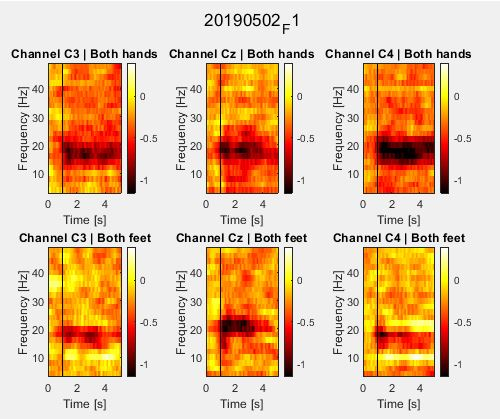
\includegraphics[width=0.5\textwidth]{Figure/20190502_ERDERS.JPG} &   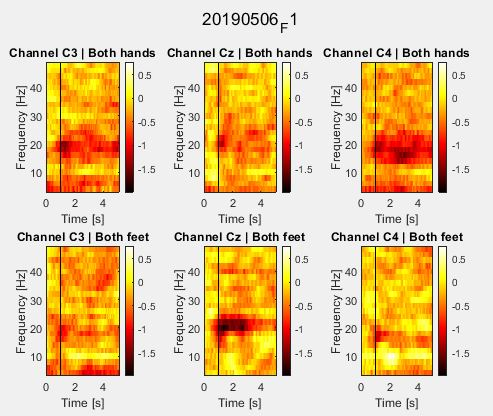
\includegraphics[width=0.5\textwidth]{Figure/20190506_ERDERS.JPG} \\
    (a) 20190502 & (b) 20190506 \\
    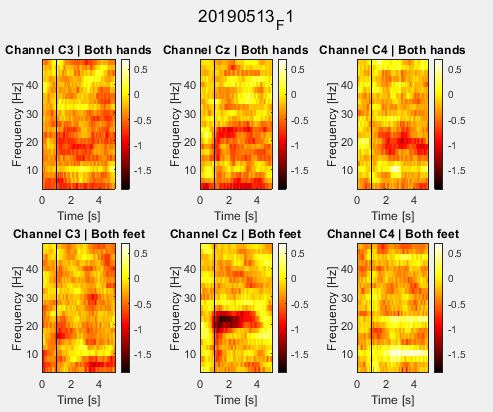
\includegraphics[width=0.5\textwidth]{Figure/20190513_ERDERS.JPG} &   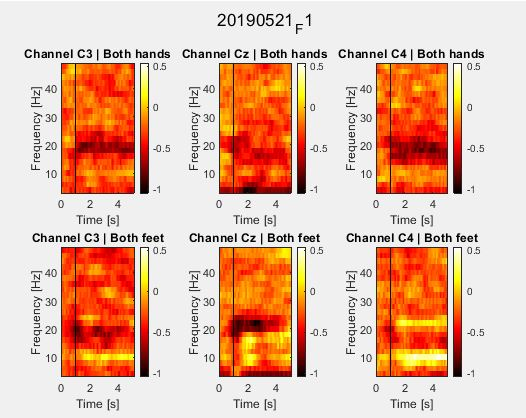
\includegraphics[width=0.5\textwidth]{Figure/20190521_ERDERS.JPG} \\
    (c) 20190513 & (d) 20190521 \\
    \multicolumn{2}{c}{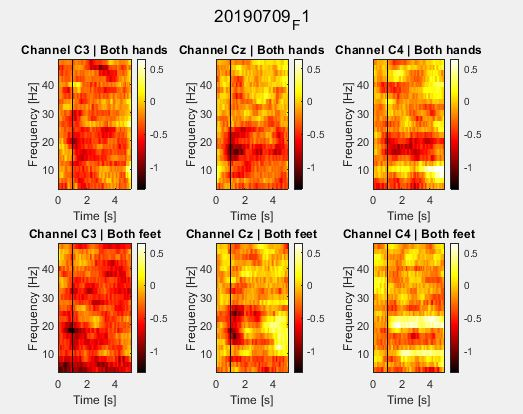
\includegraphics[width=0.5\textwidth]{Figure/20190709_ERDERS.JPG} }\\
    \multicolumn{2}{c}{(e) 20190709}\\


\end{tabular}
\caption{PSD Plots}
\end{figure}

\subsection{Fisher Score results}\label{subsec:status}
From the fisher score result is possible to highlight good discriminant between desired imagery motor in frequency 22Hz and from FC2 and C4 signals. Considering single case we can consider other frequencies like 20Hz and 18Hz and Channels Like FCZ. But this discriminant are present only in some runs, differently from C4,FC2 on 22Hz that are almost present in each offline calibration sessions. (Figure 4)

\subsection{Classifiers}\label{subsec:status}
Follows the classifier results after training. Obviously we have a better discriminant on classifiers that result strong in Channels FC2,C4 on 22Hz during fisher score analysis. This is the proof that this frequency and channels is not the better choice for all sessions. (Figure 5)

\subsection{Single Classifier}\label{subsec:status}
Just for check I tried to create a single classifier using all offline sessions data, the resulting output is very bad. The pilot change on each run and the classifier of first session is completely useless on last sessions. In fact the plot show a total overlap of the features without the possibility to find a good global discriminant (Figure 3)

\subsection{Test Sessions}\label{subsec:status}
Plot of posterior probabilities over time, with 0.7 threshold, that help to understand evidence accumulation.


\begin{figure}[h]
    \centering
    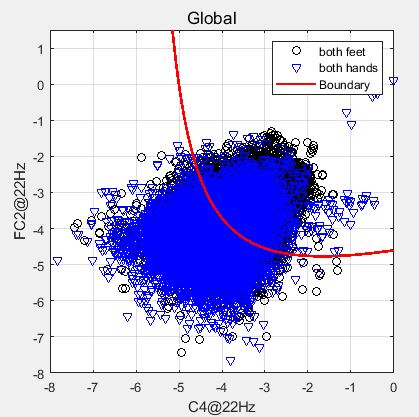
\includegraphics[width=0.5\textwidth]{Figure/GLOBAL_C.JPG}
    \caption{Single classifier.}
    \label{fig:Pipeline}
\end{figure}

\begin{figure}
\begin{tabular}{cc}
    \multicolumn{2}{c}{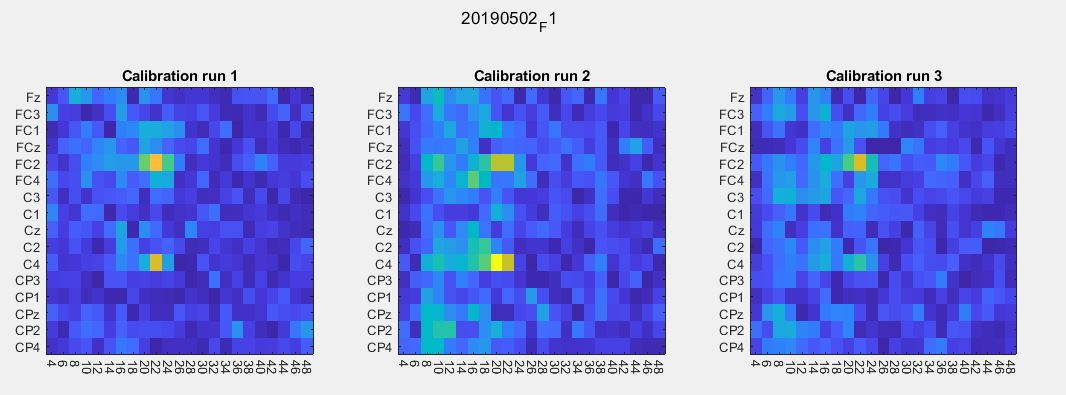
\includegraphics[width=1\textwidth]{Figure/20190502_FS.JPG} }\\
    \multicolumn{2}{c}{(a) 20190502}\\
    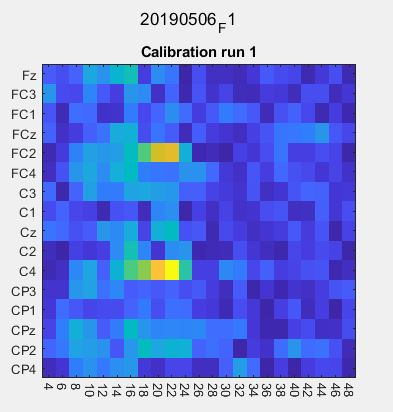
\includegraphics[width=0.5\textwidth]{Figure/20190506_FS.JPG} &   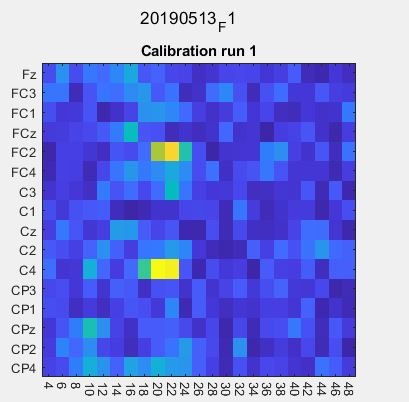
\includegraphics[width=0.5\textwidth]{Figure/20190513_FS.JPG} \\
    (b) 20190506 & (c) 20190513 \\
    \multicolumn{2}{c}{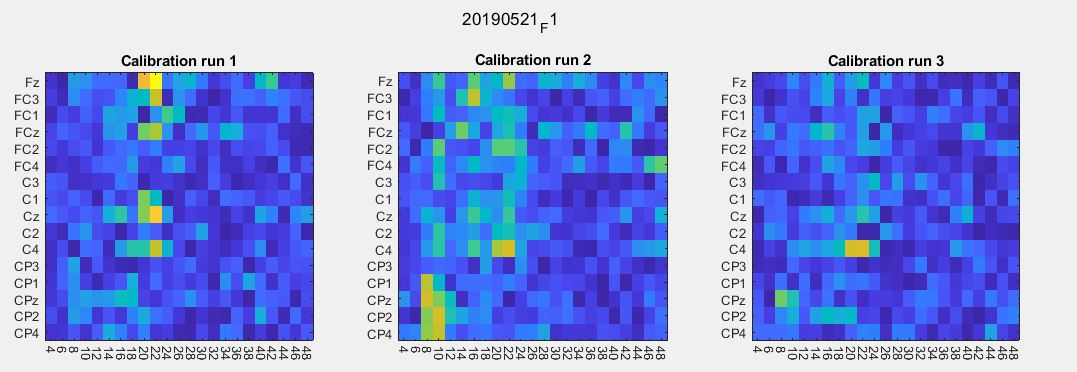
\includegraphics[width=1\textwidth]{Figure/20190521_FS.JPG} }\\
    \multicolumn{2}{c}{(d) 20190521}\\
    \multicolumn{2}{c}{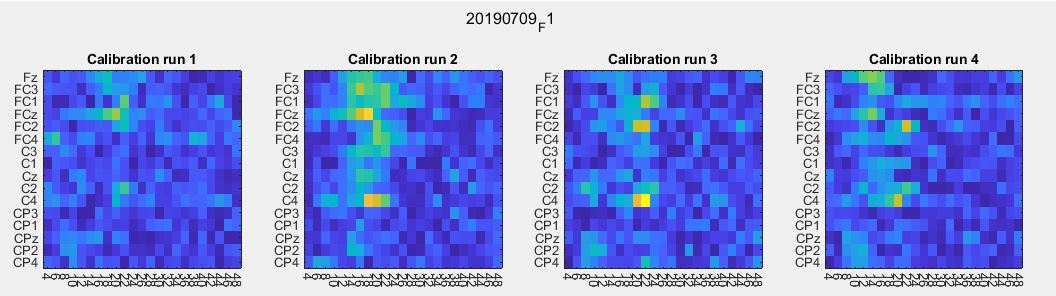
\includegraphics[width=1\textwidth]{Figure/20190709_FS.JPG} }\\
    \multicolumn{2}{c}{(e) 20190709}\\

\end{tabular}
\caption{Fisher score results}
\end{figure}




\begin{figure}
\begin{tabular}{cc}

    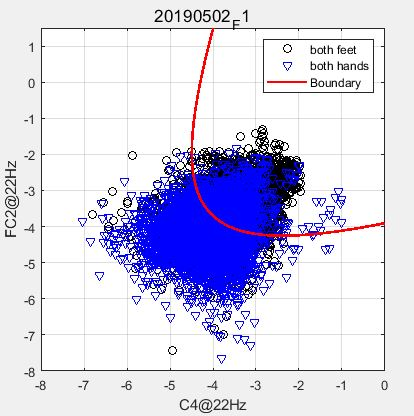
\includegraphics[width=0.5\textwidth]{Figure/20190502_C.JPG} &   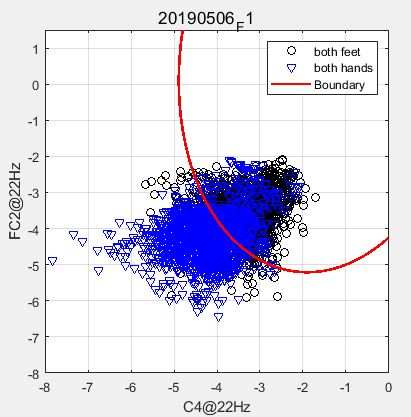
\includegraphics[width=0.5\textwidth]{Figure/20190506_C.JPG} \\
    (a) 20190502 & (b) 20190506 \\
    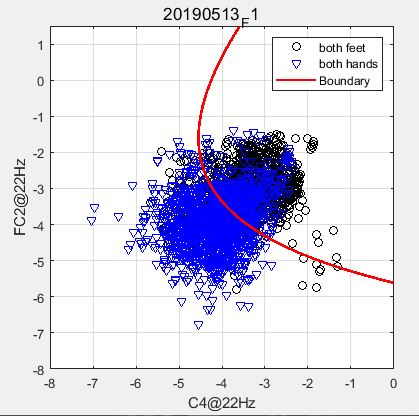
\includegraphics[width=0.5\textwidth]{Figure/20190513_C.JPG} &   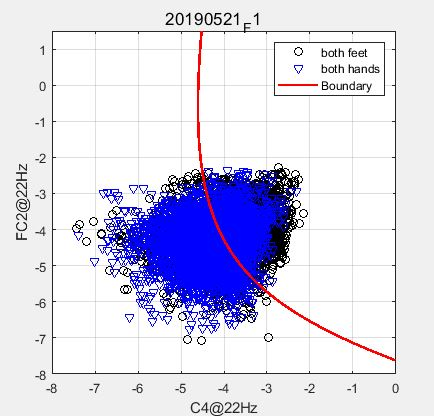
\includegraphics[width=0.5\textwidth]{Figure/20190521_C.JPG} \\
    (c) 20190513 & (d) 20190521 \\
    \multicolumn{2}{c}{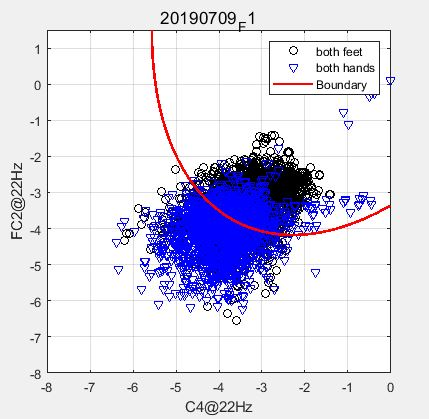
\includegraphics[width=0.5\textwidth]{Figure/20190709_C.JPG} }\\
    \multicolumn{2}{c}{(e) 20190709}\\


\end{tabular}
\caption{Models}
\end{figure}





\begin{figure}
\begin{tabular}{ccc}

    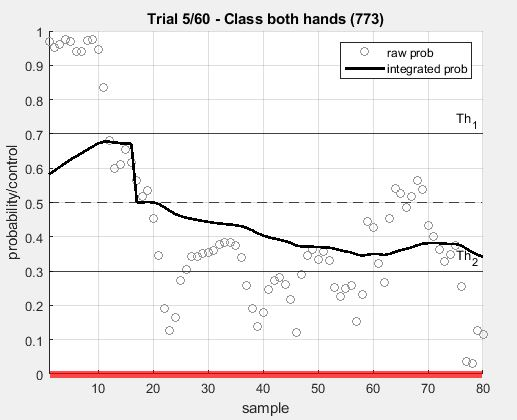
\includegraphics[width=0.3\textwidth]{Figure/20190502_F.JPG} &   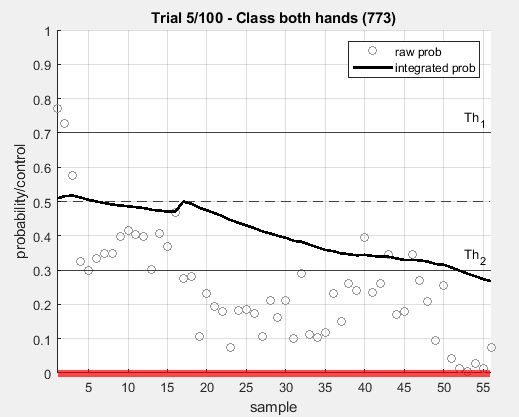
\includegraphics[width=0.3\textwidth]{Figure/20190506_F.JPG}  &   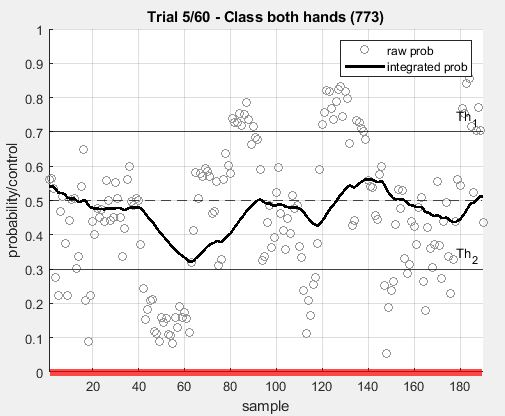
\includegraphics[width=0.3\textwidth]{Figure/20190513_F.JPG} \\
    (a) 20190502 & (b) 20190506 & (c)20190513\\
    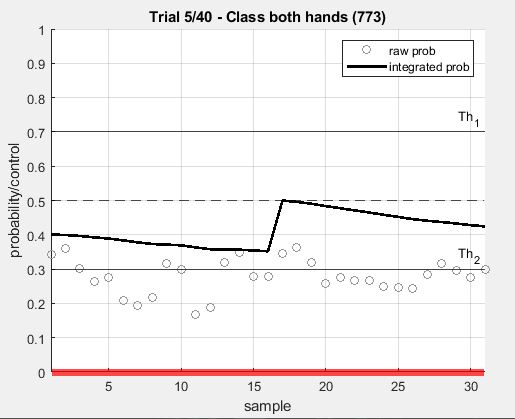
\includegraphics[width=0.3\textwidth]{Figure/20190521_F.JPG} &   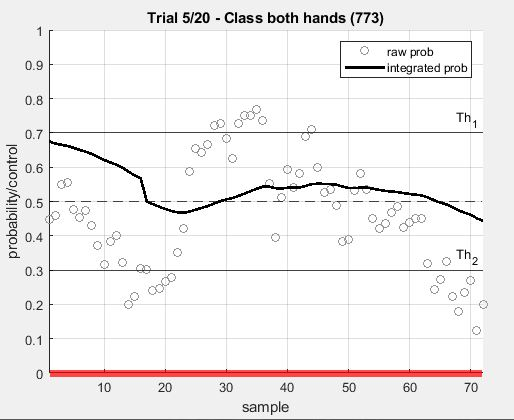
\includegraphics[width=0.3\textwidth]{Figure/20190610_F.JPG}  &   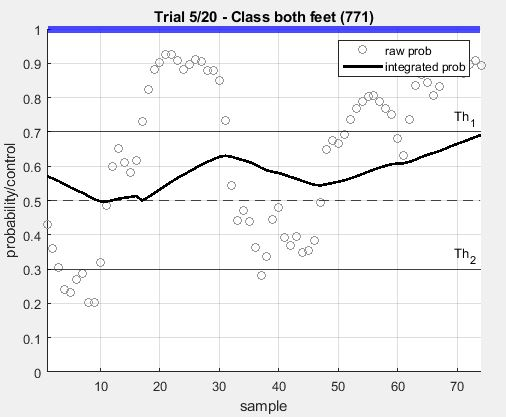
\includegraphics[width=0.3\textwidth]{Figure/20190624_F.JPG} \\
    (d) 20190521 & (e) 20190610 & (f) 20190624 \\
    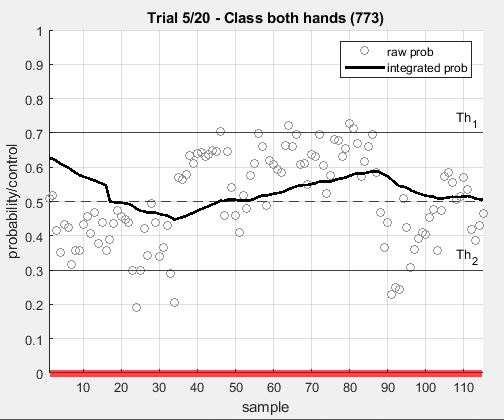
\includegraphics[width=0.3\textwidth]{Figure/20190627_F.JPG} &   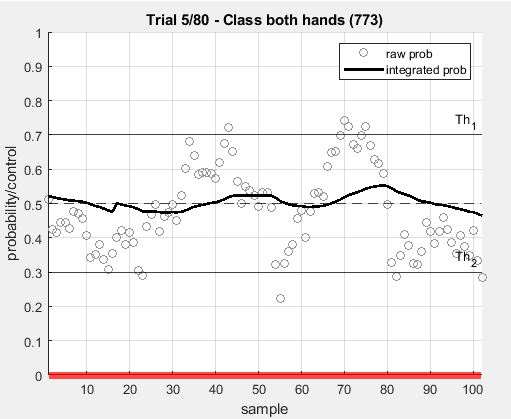
\includegraphics[width=0.3\textwidth]{Figure/20190701_F.JPG}  &   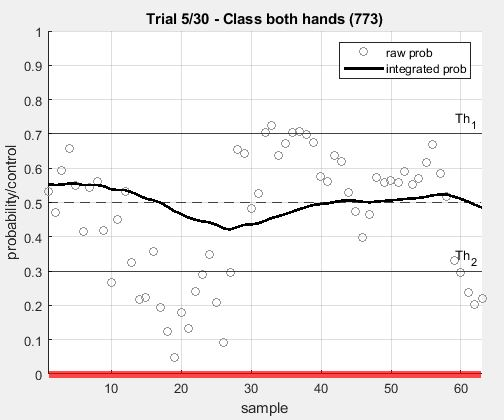
\includegraphics[width=0.3\textwidth]{Figure/20190709_F.JPG} \\
    (g) 20190627 & (h) 20190701 & (i) 20190709 \\
    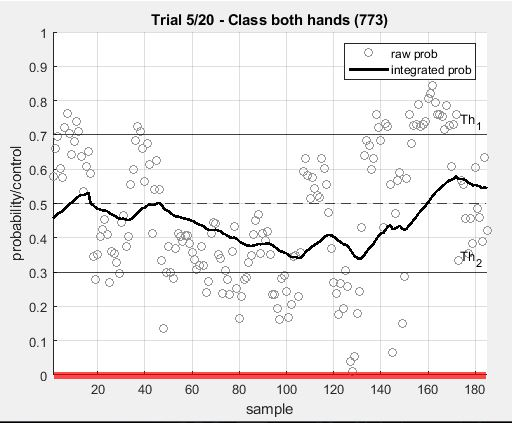
\includegraphics[width=0.3\textwidth]{Figure/20190711_F.JPG} &   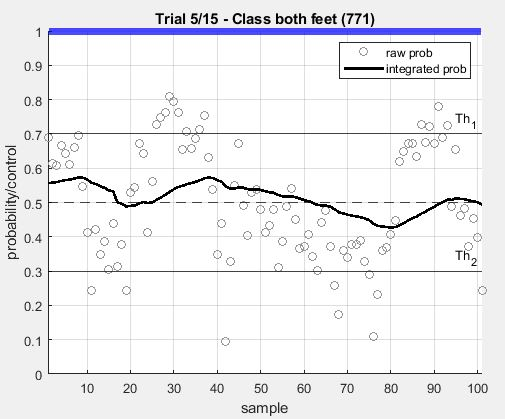
\includegraphics[width=0.3\textwidth]{Figure/20190715_F.JPG}  \\
    (g) 20190711 & (h) 20190715 \\


\end{tabular}
\caption{Models}
\end{figure}






	
\newpage
\section{Discussion}\label{sec:target_of_the_project} 
In this section we'll discuss the result obtained at the end of the pipeline, splitting the analysis in three steps, in the first step we'll discuss about results on feature selection task, on the second step the discussion will focus on classification task, and the conclusion step will discuss about the evolution of the results and performance over time.
\subsection{Feature selection}\label{subsec:status}
Feature selection task over time highlight an alternations between dominant discriminant. The main dominant channels is FC2 and C4, but not always is the best choice for classifier. As example in session 20190502, the first run highlight FC2 and C4 on 22Hz, but at third run the discriminant on C4 is weak, and during the second run we can observe some movements in 20Hz band. This situation is also observable on 20190506 runs, where the beahaveior is similar at the second run of previous session.
This uncertainty continues to recur in subsequent sessions, making it difficult to identify a unique discriminant valid for all sessions. Also in some sessions, such as the second run of the 20190709 session, where the fischer score highlights the presence of discriminants around the FCz channel on lower frequency bands between 12Hz and 18Hz. Certainly the univocal choice of channels and a common frequency band simplifies the operations but strongly penalizes some sessions, in which there is no strong discrimination between the selected channels and frequencies.
\subsection{Classification}\label{subsec:status}
As explained in the previous step, the choice of a discriminant common to all the sessions penalized all those that after each run presented discriminants distant from the common ones. Or all the sessions in which between the various runs presented a large variance in the fisher score.
All the graphs representing the classifiers are able to give a minimum separation. But unfortunately without guaranteeing the efficient separation that we would have obtained using an ad hoc feature selection tailored to each single session. Absolutely useless to try with a single classifier, it would certainly enrich the large dataset, but without taking into account the evolution over time. 
As a consequence, the results obtained in the testing phase fail to give strong evidence, despite the fact that the threshold set at 0.7 is not stringent as a parameter.
\subsection{Evolution over time}\label{subsec:status}
The strength of a static learning system is the invariance of the subject over time. In this case the learning adapts to the subject, and at the same time during the online sessions it is the same subject to adapt to the learning model.
This makes the learning process more complex across sessions, the data used for the previous models become of little use to the development of the current one. The evolution and the great variance between the various offline sessions after the sessions with feedback, demonstrates how the pilot, helped from feedbacks, adapts to the model. The real difficulty and the big difference with reinforcement learning is that with each change of the pilot, the previously acquired data cannot always be used for the train of the new model. Especially during the month of June where there were few offline sessions, we were able to observe the strong changes during the feature selection, that required a recalibration. And above all highlighted the need to carry out both types of sessions continuously, in order to prevent similar gap between one session and another. Avoiding that the patient with online-only sessions, adapting to the model introduces new features that cause loss of precision in the current model.









	


\newpage
%%% Appendici %%%
% Eventuali appendici vanno qui. Se non avete appendici da inserire, togliete/commentate queste righe.
%\appendix
%\section{Appendice A}\label{app:Appendice A}
\lipsum	

\end{document}

% Credits: basato sulle relazioni di laboratorio di Nicola Bellucco, Marco Codato e Erica Korb.